\documentclass{scrreprt}
% coma version of report class:
% http://tex.stackexchange.com/questions/5948/subtitle-doesnt-work-in-article-document-class

\usepackage{fullpage}
\usepackage[utf8]{inputenc} % åäö
\usepackage{hyperref}
\usepackage{enumitem}
\usepackage[toc]{glossaries}
\usepackage{xcolor}
\usepackage{listings}
\usepackage{tikz}
\usetikzlibrary{calc, fit, shapes.geometric, arrows}
\pgfdeclarelayer{background}
\pgfdeclarelayer{foreground}
\pgfsetlayers{background,main,foreground}
\usepackage[T1]{fontenc}
\usepackage{ulem}
\usepackage{fancyvrb}
\usepackage{shorttoc}
\usepackage{epigraph}
\usepackage{amsmath}
\usepackage{relsize}


\renewcommand*\contentsname{Contents (detailed)}


% Info about natbib:
% https://www.sharelatex.com/learn/Bibliography_management_with_natbib
% http://en.wikibooks.org/wiki/LaTeX/Bibliography_Management#Natbib
\usepackage[round]{natbib}
\bibliographystyle{plainnat}



\setkomafont{disposition}{\normalfont\bfseries}


% Remove date
\date{2014}

\hypersetup{
  colorlinks = true,
  linkcolor = black,
  citecolor = red
}

\title{ A language for expressing \\ descriptive markup languages }
\subtitle{A holistic response to constant \\ change in contemporary authorship.}
\author{ Christopher OKHRAVI \\ UPPSALA UNIVERSITY }


%
% Defining research questions
%
\newcommand\researchquestionformat[1]{\begin{quote}#1\end{quote}}
\newcommand\firstresearchquestion{\researchquestionformat{%
  \textbf{(RQ1) Research question 1} \\
  Can the verbosity of document annotation formats (e.g. \texttt{XML}) be decreased, by allowing authors themselves to design annotation formats?%
}}


\newcommand\secondresearchquestion{\researchquestionformat{%
  \textbf{(RQ2) Research question 2} \\
  Can an annotation language
  For an author to be able to design an annotation language, this author must design a domain-specific-language (DSL), a parser, a compiler and a transformation engine. Consequently we come to the point where we instead ask ourselves the following question:


  Can a \texttt{Domain Specific Language (DSL)} be defined, such that a semi-technical author can employ it to design a document annotation format?

  Requiring (A) the combined complexity of the DSL and the annotated document is less than that of a document annotated in a traditional markup language with fixed syntax (e.g. \texttt{XML}).

  Without (B) sacrificing any flexibility of the original markup language.
}}

\newcommand\thirdresearchquestion{\researchquestionformat{%
  \textbf{(RQ3) Research question 3} \\
  Can a process be defined, such that any document can be converted into \texttt{XML} format, using \texttt{Regular Expressions} as rules for document hierarchy?
}}

\newcommand\fourthresearchquestion{\researchquestionformat{%
  \textbf{(RQ4) Research question 4} \\
  Can a language be defined, such that it is a subset of \texttt{Regular Expressions}, where most control characters are replaced by assumptions? Where the intent of the subset is to express annotations of document hierarchy.
}}


\newcommand{\tab}{\hspace*{6pt}}
\newcommand{\tabb}{\tab\tab}



\newenvironment{example}
{ \hrulefill \vspace{12pt} \\ }
{ \\\\ \vspace{12pt} \hrulefill }


\lstset{
  language=XML,
  basicstyle=\color[rgb]{0.3,0.3,0.3}\ttfamily\scriptsize,
  backgroundcolor=\color[rgb]{0.98,0.98,0.98},
  showstringspaces=false,
  breaklines,
  breakatwhitespace,
}





%
%
%
% FANCY CHARACTERS
%
%
%
\newcommand*{\prim}{\ensuremath{\prime}} % Prime









%
%
% GLOSSARY
%
%

\newglossaryentry{document authoring}{
  name={Document Authoring},
  description={The act of writing literature.}
}
\newglossaryentry{EBNF}{
  name={EBNF},
  description={Extended Backus-Naur Form}
}
\makeglossaries







%
%
%
% TiKZ Figures
%
%
%
\tikzstyle{startstop} = [rectangle, rounded corners, minimum width=3cm, minimum height=1cm,text centered, draw=black, fill=red!30]
\tikzstyle{io}       = [trapezium, trapezium left angle=75, trapezium right angle=105, minimum width=2cm, minimum height=1cm, text centered, draw=black, fill=blue!30]
\tikzstyle{process}  = [rectangle, minimum width=2cm, minimum height=2cm, text centered, draw=black, fill=orange!30]
\tikzstyle{decision} = [diamond,   minimum width=2cm, minimum height=2cm, text centered, draw=black, fill=green!30]
\tikzstyle{arrow}    = [thick,->,>=stealth]
\tikzstyle{dotbox}   = [draw, dotted, rectangle, rounded corners]













\begin{document}

\maketitle
\shorttoc{Contents}{1} % Only sections
\tableofcontents
\pagebreak





% % % % % % % % % % % % % % % % % % % % % % 
%
%
%
%    The linguistic note
%
%
%
% % % % % % % % % % % % % % % % % % % % % %
\chapter*{A linguistic note}
A linguistic note in the spirit of Scribe (1980).
 






% % % % % % % % % % % % % % % % % % % % % % 
%
%
%
%    Glossary
%
%
%
% % % % % % % % % % % % % % % % % % % % % %
\glsaddall
\printglossary






% % % % % % % % % % % % % % % % % % % % % % 
%
%
%
%     Background
%
%
%
% % % % % % % % % % % % % % % % % % % % % %

\chapter{Background}

Since the invention of the writing on the wall, mankind has struggled with an interesting problem of change. Be it change in medium or means (e.g. the process of production or the means of storage). Every generation bear the burden of passing the collective body of knowledge on to the next. Every generation that cause medium or means of the written word to significantly change --  face a somewhat trivial dilemma. To somehow transcend (transform) all existing written content to fit the new ways of today, or leave the currently collected body of human knowledge to slowly perish with time.

The writing in stone cannot possibly accommodate all of the existing human knowledge. This problem of space can for example be solved by moving content to books. Paper, however, is a biological material that deteriorate with time. Consequently we have a problem of degradation. Digital representations is utterly superior in that it can be almost instantly copied and duplicated. Consequently, a process of duplication may be sufficiently cheap so as to answer to the problem of material deterioration. Because of course, even hard drives, and flash disks deteriorate with time. In the digital world however, we face a problem of interoperability. New file formats are invented every day. Employing a naive process of constant duplication will leave our future selves in a position where some formats may be as costly to interpret as the ancient writing on the wall is to us today. As the native speakers of a language die, so does the knowledge uniquely encoded in that language.

Instead, I argue that the one sensible approach is to employ a constant rewriting of the complete body of written human knowledge. To ensure that no authored work is lost in the translation of time.

But the big problem is of course that this is an utterly massive undertaking. So massive that it is obviously absurd to assume this process should be carried out by humans. But not yet so massive that it would be absurd to ask computers to carry it out. This thesis suggests taking a holistic approach to the current body of markup languages, identifying the common intersection, and suggesting a structured way in which some subset of languages any of these languages can be transformed into any of these other languages (TODO! THIS IS NOT CORRECT). With less human effort required than today. And with more preparation for potentially new languages of the future.

\paragraph{TODO}
- A brief history of writing from pens, to the printing press, to computers and word processors, to markup languages.
 




\section{Problem outline}
\label{sec:problems}
The problem area of this thesis is probably best be summarized by a quote raised in a paper by \cite*{krijnen} on a different approach to a problem similar to the problem raised in this thesis.

\begin{quote}
``The nice thing about standards is that there are so many to choose from.''\\
\textit{-- Andy Tanenbaum}
\end{quote}

Because we have so many different formats, for various good reasons, the need to convert between these formats, for various good reasons, is apparent. Let us begin with some examples. A reason for why we have different input formats may be that we as individuals appreciate different approaches and ways of thinking and thus syntaxes. Another might be that some formats simply cannot express concepts that another format can express. A reason for why we would like to convert between formats could be that of publishing. Given the multitude of devices and programs that can consume our documents it should be in our interest to supply appropriate formats for these devices and programs. 

\paragraph{Call this the ``n-to-n conversion problem''} (or simply ``n-to-n''). An existing approach to this ``n-to-n'' conversion problem, and perhaps the most obvious one, is Pandoc\footnote{http://johnmacfarlane.net/pandoc/} -- dubbed ``a universal document converter''. The problem I see with Pandoc however is it's lacking facilities for customization of the conversion process. Assume for example that we are converting a document expressed in Markdown to HTML. None of the formats natively support the concept of a Table Of Contents (TOC). Wanting to do this, we would have to ``intercept'' the program after it has parsed the input, and use Haskell or Python to transform the JSON representation of the Abstract Syntax Tree (AST). This interception possibility is not a ``hack'' but built in to the Pandoc system and referred to as Scripting\footnote{http://johnmacfarlane.net/pandoc/scripting.html}.

Thus, the issues related to Pandoc are two-faceted. On one hand (P1) it may be difficult for semi-programmers to significantly modify the structure of a output document, but on the other -- even (P2) assuming programmers would collectively build an extensive library of transformation scripts for Pandoc, these ``packages'' operate on AST's that represent already complex formats. This facility and it's drawbacks is made clear in the research of \citet{krijnen}, who propose a solution for essentially the same problem as this thesis. The main difference between the approach of this thesis and that of \citet{krijnen} is that they operate on a ``lower level''. Seemingly \citet{krijnen} operate with intents of compilation efficiency through the use of lazy-evaluation, and criticize the Pandoc scripting system for requiring multiple (thus costly) runs over the AST. While the work of \citet{krijnen} is splendid, I unfortunately argue that formal grammars are too complex for such a tool to be used by laymen, or semi-programmers.
%TODO: Make the P's and their problems more clear. Why are they never referred to?

To put this thesis in relation to Pandoc's Scripting facilities, the argument goes along the lines of readability for the masses. I am not arguing that the current approach of Pandoc is absurd -- in fact, argue the approach of \citet{krijnen} is beautiful from a composition point of view, and I argue that the approach of Pandoc is effective in getting around to solve the problem without too much fuss. In this thesis, we will however look at an approach I argue is even more fuss-free than that of Pandoc Scripting. This is why we talk about a holistic approach to markup languages. Subjectively I would argue that both Pandoc and the work of \citet{krijnen} are \emph{reactive} instead of \emph{proactive}. In this thesis we look at the intents of markup languages from a more abstract point-of-view, revisit the actual intents and needs and not simply argue that the problem is the need to convert all formats to all formats. That undertaking, I argue, is too huge to provide significant value -- yet (TODO -- unclear).

\begin{quote}
``If I had asked people what they wanted, they would have said faster horses.''
\begin{flushright}
% TODO Make sure all quotes are formatted alike
\textit{-- Commonly attributed to Henry Ford}
\end{flushright}
\end{quote}


\paragraph{Consider instead a ``1-to-n'' problem}. Expressing our documents in a single format but converting into any imaginable format. This approach has been utterly popularized and democratized through the family of languages under XML. If one considers the scenario where an author choose to always express documents in the one format and never in any of the family of n -- then one could argue that solving this problem also solves much of the intent of the ``n-to-n-problem''.

An author can express her document in an arbitrary XML-format (perhaps imagined ``on the fly''), and then use a combination of XSLT and XPath to convert this document into any other imaginable format. Some problems with this approach is (1) the verbosity of the XML languages\footnote{http://www.ibm.com/developerworks/xml/library/x-sbxml/index.html} \footnote{http://blog.codinghorror.com/xml-the-angle-bracket-tax/} \footnote{http://blog.codinghorror.com/revisiting-the-xml-angle-bracket-tax/}, and (2) the fact that because of the lack of any kind of centralization or standardization of format or process, reuse of common transformations become difficult. The composition problem becomes apparent again. Wouldn't you rather use an XML to PDF transformer that the community had curated rather than rewriting one from scratch? Rhetorical question. The problem is again that since XML allows for an infinite number of syntaxes it is non-trivial to encompass all these syntaxes in the transformer.

\paragraph{Of course there are XML subsets like DocBook} that are more commonly accepted than others. Thus, community curated packages exist that can convert between the commonly used format and some other common presentational format e.g. PDF\footnote{http://docbook.sourceforge.net/}. This makes the XML situation look very much like the Pandoc situation (TODO -- not entirely) but instead of considering completely different syntaxes as input, one considers the XML-based languages. The main problem with this approach is that the input format is fixed. If (e.g.) the Docbook format is not sufficiently rich to express some concept that the author want to express then the community curated converter will be of limited use. Thus, that is a problem with diverging input. In the other end, we can look at diverging output. If working with standards, it is reasonable to assume that there is a standardized (or set of standardized options) for output. What if the author wishes to diverge from the standard output style? How much is flexible and configurable?

\paragraph{Instead} this thesis suggest to employ a view of \texttt{M-to-N}, where \(number\_of\_languages\_in(M) < number\_of\_languages\_in(N)\). Where \(M\) is the body of  languages imagined by authors, declaratively expressed at the highest level of abstraction possible for the given domain, and \(N\) is the set of all potential languages the author might want to convert the input into. Where all languages in \(M\) must lie in the intersection of all the languages in \(N\). In other words \texttt{\(M \subset (N_1 \cup N_n) \)}. 

In this thesis I will argue that there is a difference between converting a document when the language is within M, from M to N, or within N. I will also argue that employing this division will spawn much more pragmatic solutions than many-to-many-document conversions.

\paragraph{The aim} of this thesis, is to suggest a software eco-system\footnote{TODO -- need to define term?} in which a document author can ``write once, [and] publish everywhere''. But of course, that is an oversimplification. More specifically this thesis suggest a way in which we could write our (1) actual document contents once, (2) the transformation process in which we create, what \citet{reid} refers to as, ``derived text'' once, and finally (3) the mapping onto an output format once (per format of course). Note that the two second parts are generalized, and could be published as packages and reused. Note also that the manually authored files at each step are merely configuration files. Between each above step lives a compiler, and these compilers are \emph{not rewritten} on a per-conversion-basis. What also is not obvious in the above explanation is that this thesis suggest an approach that can be likened by a pipeline of templates (similar to a UNIX pipe\footnote{http://en.wikipedia.org/wiki/Pipeline\_(Unix)}) and through this achieve a high level of composability. Instead of a one-pass-transform, transformations are split into composable chunks at different levels of abstraction. But all this will be discussed further on in the thesis.






% TODO: Use or remove?
%\paragraph{Existing solutions}
%\begin{itemize}
%\item No proper pipeline for reusing common things, such as the creation of a table of contents.
%\item Could be solved using e.g XSLT but too verbose. No standard way of sharing libs.
%\item Pandoc is too difficult to configure. Syntax. Haskell/Python. Lacks an approach to share libs. 
%\end{itemize}



\section{Requirements}
Given the holistic problem outlined in Section \ref{sec:problems}, we will discuss a holistic response, in form of an eco-system of tools. In order to guide the development of the tool-chain, the following requirements have been extracted from the problems outlined in Section \ref{sec:problems}.

\paragraph{Any output format but reasonable input format}
As an author I must be able to author my document once, in a ``reasonable'' format. However, as an author, I must be able to publish to multiple platforms -- without \emph{any} rewriting. However, minor configuration must be allowed in order to ensure flexibility in output.

\paragraph{Composable} or code reuse through package friendliness. Code reuse must be a top priority. Not merely within an author's workflow of a single document, but also between authors and documents. Consequently, as much as possible must be able to be distributed as packages. \footnote{TODO -- call it composability or modularity?}

\paragraph{Extendable} refers to the idea that it must be natural to introduce new packages that intercept the process at any point in time. This requirement encompass the idea that authors must be offered control over the production of the final output.

\paragraph{Declarative}
All code that an eco-system user would touch must be declarative. Also packages must be expressed declaratively. This encompass the idea of using template transformations rather than imperative processing.




\section{Thesis outline}
TODO.



























% % % % % % % % % % % % % % % % % % % % % % 
%
%
%
%     Theory
%
%
%
% % % % % % % % % % % % % % % % % % % % % %


\chapter{Theory}
TODO.



\section{A brief history of Markup}

- What does it mean to annotate? What are common document annotation formats?

- Examples of markup languages and showcase of some syntax examples.

- A brief overview of markup languages and how they can be used for (1) Document authoring, and (2) Data transport.

- The relevance of markup for fiction and non-fiction.








\section{Nested markup}
A fundamental feature of (many) descriptive markup languages is the ability to nest elements such that a larger set of semantics is expressable than with merely the isolated elements themselves. In most descriptive markup languages, this is implemented as the ability to nest elements in order to create hierarchies. As \citet*{durand} point out, describing documents as ordered hierarchical structures, is the view that has been most prominent. Perhaps because there exist many conflicting suggestions on how to approach non-hierarchical documents. Some of these are outlined by \citet{durand} but an extensive amount of papers have been written on the subject matter\footnote{http://xml.coverpages.org/hierarchies.html}. Even today, hierarchical document structures enjoy the most widespread use. Consider, for example, the large family of XML-based languages such as HTML.



To enforce the difference between nesting and not, consider the following example. Assume we have a formatted paragraph of text\footnote{In this example we will disregard whitespace between tokens and assume that whitespace between words in a string remains, but whitespace between strings is omitted and left implicit.}, as outlined in Figure \ref{fig:mixed-content-paragraph}.


\begin{figure}[h]
\centering
\fbox{
The color \underline{is \textbf{now}} \sout{red}.
}
\caption{An example paragraph with formatting.}
\label{fig:mixed-content-paragraph}
\end{figure}


Assume that we want to mark up some aspects of the formatting. The important\footnote{...and admittedly fabricated...} characteristics are that the paragraph, from a markup perspective, can be argued to consist of four unique ``token types''. More precisely (1) plain-text, (2) underline, (3) bold-underline, and finally (4) strikethrough.





\begin{figure}[h]
  \centering
  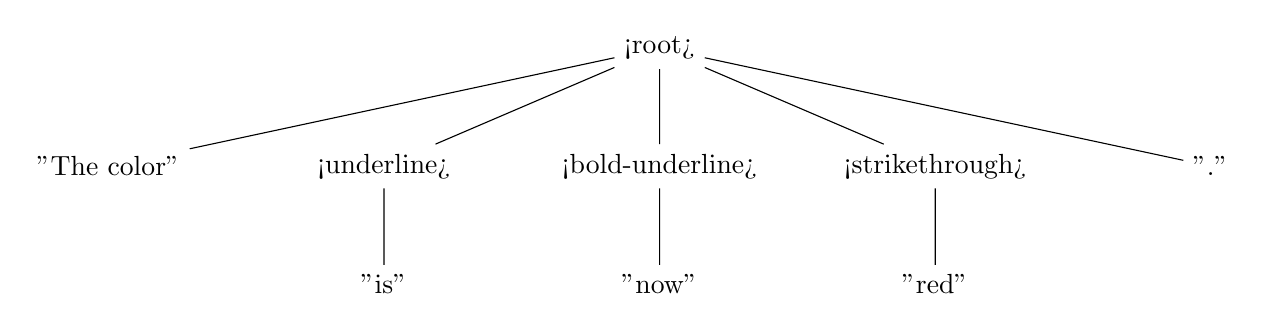
\begin{tikzpicture}[
    tlabel/.style={pos=1,right=2pt,font=\footnotesize\color{red!70!black}},
    sibling distance=3.5cm,
  ]
  \node {<root>}
  child {node {"The color"}}
  child {node {<underline>}
    child {node {"is"}}
  }
  child {node {<bold-underline>}
    child {node {"now"}}
  }
  child {
    node {<strikethrough>}{
      child {node {"red"}}
    }
  }
  child {node {"."}}
  ;
  \end{tikzpicture}

  \caption{Pre-order tree representation of Fig. \ref{fig:mixed-content-paragraph}.}
  \label{fig:mixed-content-flat-tree}
\end{figure}



More importantly, the fact that two words are underlined, whereas one of the words that are underlined is actually both underlined and bold. This is an example of a situation where nesting may help us express a string more efficiently. Consider the difference between the non-nested tree representation in Figure \ref{fig:mixed-content-flat-tree} and the nested tree representation in Figure \ref{fig:mixed-content-tree}. In the example that employ nesting, we are actually re-using the semantics of one string to partially describe another.


\begin{figure}[h]
  \centering
  \begin{tikzpicture}[
    tlabel/.style={pos=1,right=2pt,font=\footnotesize\color{red!70!black}},
    sibling distance=3cm,
  ]
  \node {<root>}
  child {node {"The color"}}
  child {node {<underline>}
    child {node {"is"}}
    child {node {<bold>}
      child {node {"now"}}
    }
  }
  child {
    node {<strikethrough>}{
      child {node {"red"}}
    }
  }
  child {node {"."}}
  ;
  \end{tikzpicture}

  \caption{Pre-order tree representation of Fig. \ref{fig:mixed-content-paragraph} employing nesting.}
  \label{fig:mixed-content-tree}
\end{figure}



To understand why nesting is a sensible approach to such situations consider the lexing step of a compiler that read the paragraph in question. Without nesting, the number of terminal tokens needed in the lexer would have to be a number that exponentially increase with every introduced new terminal token, because tokens can be combined with tokens.






\subsection{Arguing the case of nesting}
I argue that nested markup is a fundamental, and necessary property of any pragmatically useful markup language. I will make four arguments in order to support the use of nesting. First I will argue that (1) there is no semantic difference between an element implied by the use of nesting rather than it's explicit counterpart. Secondly, I argue that (2) no significantly complex cognitive leap is required for humans in order to be able to think and discuss nesting. The two remaining arguments enforce the power of nesting. (3) Nesting can reduce the number of required terminal tokens in a markup compiler exponentially. Finally, (4) nesting allow languages to contain an infinite set of semantic tokens while expressing only a finite set of tokens in the compiler.

The arguments will be explored in some detail below.



\paragraph{(1) No semantic difference.}
Other than explicitness, whether a particular string (s) belong to a particular semantic domain (D) is of course constant regardless of what syntax is used to express its belonging. Consider the classic saying ``syntax is not semantics''. Nesting is simply a form of context-sensitive syntax. A form of implicit syntax rather than explicit.

Consider for example chapters and subchapters. One explicit way of distinguishing between the two would be to introduce one syntactic keword denoting a chapter, and another denoting a subchapter. This is an explicit approach. An implicit approach however would be to argue that any chapter ``inside'' of another chapter should be considered a subchapter. In this latter case, only the syntactic keywords for denoting a chapter are required.

One may of course argue that there is a subtle difference between a chapter in a chapter, and a subchapter. That would however be to misinterpret the point. Think not in terms of defining a one, true, global language that encompass all envisionable semantics. Think instead in terms of one author defining her own syntax denoting some semantics envisioned by her. If the author claim the implicit syntax is the same as the explicit syntax then there is no point in arguing differences in specific cases. The author has only claimed that the implicit syntax and the explicit syntax are the same in her particular case.

Thus, I argue, that there is no reason write off nesting with arguments of subtle semantic differences. Simply because the author of a language have all the right to couple any kind of semantic to any kind of syntactic construct. Regardless of whether the syntactic construct is context-free or context-sensitive.




\paragraph{(2) No significantly complex cognitive leap.}
TODO: This is actually a really poor argument. It's probably the other way around. Put this as critique instead. Think of the 32-nested stars-example.





\paragraph{(3) Nesting reduce the number of terminal tokens.}

Assume two unique terminal tokens -- \(A\) and \(B\). Assume a language where a string can belong to either the class A, or the class B, or simultaneously to the class of both A and B. Without the power of nesting, this requires the introduction of a third explicit token -- call it \(C\). Understand that we started out with two initial unique tokens, and that through allowing these tokens to be combined, we were forced to introduce yet another token in order to be able to encode this ``combined'' token.

Now, understand that the above example only require the introduction of one more token, because the starting point consist of a set of (merely) two unique terminal tokens. You may have realized, that introducing single token, is not sufficient if the starting point is a set of three unique terminal tokens. Subsequently far from sufficient if the starting point is a set of 100 unique terminal tokens.


\begin{figure}[h]
\centering
\fbox{
Lexing \underline{without \textbf{\sout{parsing} often}} \sout{make} \textbf{life \sout{oh so} \underline{cumbersome}}.
}
\caption{Exhibiting all combinations of \{bold, underline, strikethrough\}.}
\label{fig:mixed-content-paragraph-complex}
\end{figure}


Analyzing the paragraph outlined in Figure \ref{fig:mixed-content-paragraph}, one may suspect that the underlying language can be described by a grammar consisting of the three tokens outlined in Equation \ref{eq:tokens-as-subset} where plain-text is disregarded. Mixing and matching these tokens, one can trivially create a string, such as Figure \ref{fig:mixed-content-paragraph-complex}, that indeed exhibit the need of more than merely one more terminal token.



\begin{equation}
\{B, U, S\} = \{bold, underline, strikethrough\}
\label{eq:tokens-as-subset}
\end{equation}



Mathematically, the total number of terminals in a grammar that allow combinations of unique terminal tokens, correspond to the number of k-combinations for all k, of \(n\), where \(n\) is the number of unique terminal tokens before combining. In other words: the total number of tokens is the number of possible subsets of the set of unique terminal tokens. Expressed in Equation \ref{eq:formula-all-subsets}.

\begin{equation}
\sum_{0\leq{k}\leq{n}} {n \choose k} = 2^n
\label{eq:formula-all-subsets}
\end{equation}

Since the Equation \ref{eq:formula-all-subsets} also include the empty set we would need to modify the formula such that it subtracts one. However, remember that what we are trying to calculate, is the number of terminal tokens needed to express some grammar of a language where the initial terminal tokens can be combined arbitrarily. Consider the fact that one terminal token of markup languages is plain-text. Consider also the fact that depending on the philosophical orientation of the reader, plain-text can either be considered to be combined with all combinations or none of them. It does not make sense to distinguish between a token that is plain-text-and-bold, from a token that is merely bold. They are essentially the same. In the example, plain-text will be the token that represent the unsuitability of all other tokens -- in other words: if no token match, then the token must be plain-text. Consequently, there will only ever be one combination including the plain-text token regardless of the size of \(n\) and \(k\). Thus, the empty set, in the formula above, will represent the plain-text, and thus there will be no need to subtract one.

Applying this formula to Figure \ref{fig:mixed-content-paragraph} would yield the same number of subsets as depicted in Formula \ref{eq:all-subsets-of-example}. The set used as a starting-point is depicted in Formula \ref{eq:tokens-as-subset}.

\begin{equation}
|\{\{\};\{B\};\{U\};\{S\};\{BU\};\{BS\};\{US\};\{BUS\}\}|
\label{eq:all-subsets-of-example}
\end{equation}


Following this line of thinking an interesting question may be posed. Why merely combinations and not permutations? In other words: many markup languages allow authors to permute the base tokens and not merely combine them. To emphasize the difference consider the subtle distinction between an \textit{\textbf{italicized bold}} string and a \textit{\textbf{bolded italic}} string.

Whether such a distinction would matter in a language is of course dependent on that particular language, and might even vary on a per-token-basis within that particular language. While the distinction might be irrelevant in the example above (combining bold and italics), consider instead the semantic distinction between a \emph{paragraph in a figure} and a \emph{figure in a paragraph}.

Assuming a language where all tokens may be permuted and not simply combined, the total number of tokens required in the grammar would be significantly higher than in the combinatorial case. In mathematical terms, the number corresponds to the number of k-permutations of n, for all k, where n is the number of unique terminal tokens before combining (as depicted in Formula \ref{eq:formula-permutations}).


\begin{equation}
\sum_{0\leq{k}\leq{n}} P(n,k) = 
\sum_{0\leq{k}\leq{n}} \frac{n!}{(n-k)!}
\label{eq:formula-permutations}
\end{equation}

Assuming that the language of the previously discussed paragraph (Figure \ref{fig:mixed-content-paragraph}) allow permutation of tokens. Treating the language as the set of tokens depicted in Equation \ref{eq:tokens-as-subset}, and applying the formula to that set (as depicted in Equation \ref{eq:all-tuples-calculation}), yield 16 tuples, where the tuples in question are depicted in Equation \ref{eq:all-tuples}.



\begin{equation}
\begin{split}
\frac{3!}{(3-3)!} + \frac{3!}{(3-2)!} + \frac{3!}{(3-1)!} + \frac{3!}{(3-0)!} = 
16
\label{eq:all-tuples-calculation}
\end{split}
\end{equation}



Consequently, if one has a language consisting of three original terminal tokens, and wish to construct a language where each possible k-permutation of the three tokens correspond to unique token, then the language must actually contain 16 tokens. In a language that starts with four terminal tokens, the number of actually required terminal tokens is 65. Obviously this is absurd. And thus, this is a reason as to why nesting is such an important corner stone of markup languages. Because it allow languages to omit the explicit use of terminals in favor of implicit hierarchies.




\begin{equation}
\begin{split}
\{
(); \\
(B);
(U);
(S); \\
(B,U);
(B,S);
(U,B);
(U,S);
(S,B);
(S,U); \\
(B,U,S);
(B,S,U);
(U,B,S);
(U,S,B);
(S,U,B);
(S,B,U)
\}
\label{eq:all-tuples}
\end{split}
\end{equation}


% TODO: Call these ``derived'' tokens????




\paragraph{(4) Nesting enable infinite semantics.}
This last argument can easily be understood by contemplating the language of infinitely nestable chapter tokens. In other words, a markup language in which every chapter nested inside of another chapter denotes a subchapter of the chapter level of the previous chapter. In other words the first time a chapter appears, it is a top-level chapter. When a chapter appears within that other chapter it is a sub-chapter. When a chapter appears within that sub-chapter, it denotes a sub-sub-chapter. And so forth into infinity.

Such a language can be described by allowing elements to nest, and decide upon the semantic rule, that any chapter within a chapter is a sub-chapter of that chapter. This is obviously a powerful feature, it is obviously very common in markup languages, and obviously not (trivially) expressible without nesting, in a finite grammar.







\begin{figure}[h]
\centering
\fbox{
Consider (the (infinite (nesting) of (parentheses))).
}
\caption{An example paragraph where some words are marked up in multiple ways}
\label{fig:mixed-content-nesting}
\end{figure}







\subsection{Non-hierarchical nesting}
It is important to understand that this thesis employ and endorse the hierarchical model of nesting for delimitational and pragmatic reasons. The necessary property, I argue, is nesting -- not necessarily hierarchical nesting. However, since there is disagreement in the community (as previously mentioned) on how to approach non-hierarchical nesting, it shall be left as a request for further research.











\section{Mixed content}
When discussing markup languages -- it is important to identify the sometimes subtle distinction between languages suitable for (1) \emph{data modeling} and languages suitable for (2) \emph{document authoring}. The prior is concerned with structured data, whereas the second is concerned with structured data that fit within the metaphor  of a document. As the first can be described as referring to datastructures -- one could of course argue that any imaginable document (in the document authoring sense) could be encoded in a particular data structure. Thus that there consequently could not exist any clear distinction between data oriented formats, and document oriented formats. That is however not the argument being opposed here. In order to make unambigious use of these terms in the thesis, below an explenation of one separation is explained. Essentially it encompass the idea that some languages are more suited for intermingling non-marked up text with marked up text.

% TODO: Use and refer to the terms used by H. Schöning (2001) -- Tamino a DBMS for XML.

The first official W3C working draft of XML (1996)\footnote{http:\/\/www.w3.org/TR/1998/REC-xml-19980210\#sec-mixed-content} already contained the idea of what was referred to as ``mixed content''. Simplified, the idea was that an element may either contain a string of text, or another element, or any combination of the two. In (1998) W3C published a recommended specification of XML 1.0, where the concept of mixed content was expressed as a grammar in Extended Backus-Naur Form (subsequently referred to as EBNF) as follows\footnote{Part of the production for the non-terminal ``content'' has been omitted in favor of readability.}.

\begin{lstlisting}
element ::= EmptyElemTag | STag content ETag 
content ::= (element | CharData)*
\end{lstlisting}

In essence -- any non-terminal \texttt{element} can either produce an \texttt{EmptyElemTag} (i.e. self-closing tag), or the set of a \texttt{STag} (i.e. opening tag) followed by \texttt{content}, followed by an \texttt{ETag} (i.e. closing tag). The non-terminals \texttt{start} (e.g. \texttt{<foo>}) and \texttt{end} (e.g. \texttt{</foo>}) will terminate without any risk of indirect recursion back to the non-terminal \texttt{element}. The non-terminal \texttt{content} is the one interesting to this example.

The XML 1.0 (1998) specification use the following flavored syntax\footnote{This is of course merely a partial extraction of the syntax used in the specification.} of EBNF. The character ``pipe'' (|) represent an \texttt{XOR} choice such that \texttt{A | B} match ``A or B but not both''. The character ``star'' (*) is used as a ``Kleene Star'' such that \texttt{A*} matches ``zero or more occurrences of A''. Parentheses is used to group expressions such that the two mentioned operators can be used on an expression group.

This essentially mean that the non-terminal \texttt{content} can produce either a new \texttt{element} (causing indirect recursion) or \texttt{CharData} (i.e. a string), any number of times. Subsequently allowing for any combination of any length of the two.



\subsection{Arguing the case of mixed content}
TODO: CONTENT MOVED TO NESTING




\subsubsection{Suitable formats for Mixed Content}
Figure \ref{fig:mixed-content-paragraph} in XML.


\begin{figure}[h]
\begin{lstlisting}
The color <underline>is <bold>now</bold> <strikethrough>red</strikethrough>.
\end{lstlisting}
\caption{Expressing Figure \ref{fig:mixed-content-paragraph} in XML.}
\label{fig:mixed-content-xml}
\end{figure}



\subsubsection{Unsuitable formats for Mixed Content}
Mixed content becomes utterly difficult to express in languages that lack a canonical way of expressing it. Attempting to express Figure \ref{fig:mixed-content-paragraph} in JSON, one quickly realizes there are multiple ways and that it is not obvious which was is the one to prefer. No approach I have found\footnote{I have merely conducted non-scientific experiments.} is trivial to parse without telling the parser a particular piece of information.

\begin{figure}[h]
\begin{lstlisting}
{
  "root": [
    "The color ",
    { "emph": ["is", { "keyword": "red" }], },
    "now."
  ]
};
\end{lstlisting}
\caption{Attempting to express Figure \ref{fig:mixed-content-paragraph} in JSON.}
\label{fig:mixed-content-json}
\end{figure}


Consider Figure \ref{fig:mixed-content-json}. At first glance it seems like a perfectly reasonable representation of the discussed paragraph. Using Arrays to sequence, and single-key objects to name elements. However, the limitations become painfully apparent if we ask ourselves the question -- what does an object with two keys represent?

One might argue that the counter example is breaking the rules. We did say ``single-key objects'' and not ``n-key objects''. This is a syntactical requirement that can easily be encoded into the parser (or probably even the lexer). This is however to misunderstand the point. The point is that the JSON specification does not actually enforce this behavior today. Meaning, there is (to my knowledge\footnote{TODO: Do I need a reference or something?}) no way of representing mixed content with labeled elements using JSON, without introducing a requirement that isn't already encoded in the lexer/parser. Meaning, all valid JSON strings, cannot (applying a certain strategy, such as e.g. Figure \ref{fig:mixed-content-json}) be considered valid strings of mixed content. This is visualized in Figure \ref{fig:mixed-content-venn-json}. Ergo, JSON is an unsuitable format for mixed content.

Within this thesis, it is this line of reasoning that is referred to when discussing whether a particular format is suitable for representing mixed content or not.




\begin{figure}[h]
\centering

  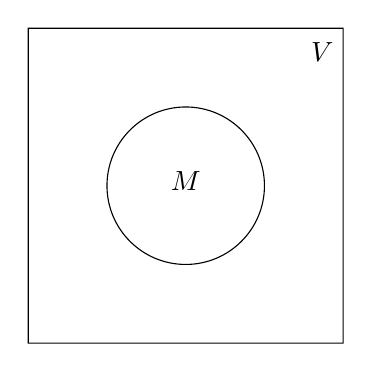
\begin{tikzpicture}[fill=gray]
  % left hand
  \scope
  \clip (-2,-2) rectangle (2,2)
        (1,0) circle (1);
  \endscope

  % outline
  \draw (0,0) circle (1) (0,1)  node [text=black,below,yshift=-.7cm] {$M$}
        (-2,-2) rectangle (2,2) node [text=black,below,left,yshift=-.3cm] {$V$};
  \end{tikzpicture}

  \caption{Venn diagram, where \(V\) is all valid JSON strings and \(M\) is all valid JSON strings that are also valid mixed content strings. }
  \label{fig:mixed-content-venn-json}
\end{figure}



\paragraph{Ambiguity in JSON mixed content}
TODO: Show examples of how lexing and parsing JSON mixed content may create different parse trees. Ambiguity.



\subsection{Enforcing the importance of mixed content}

\citet*{mignet} analyzed different aspects of what they referred to as ``The XML web'' (i.e. "the subset of the Web made of XML documents only"). During this study it was found that 72\% of all documents utilize mixed content. Almost three out of four documents use mixed content. \citet{mignet} conclude that they've invalidated the folklore of underestimating the importance of mixed content in XML. Given that XML (in contrast to HTML -- the de facto language of the web) is commonly used as a data transportation format, one can reasonably assume that the number of HTML documents making use of mixed content is even higher.



Further, anyone who has ever authored a free-text-oriented document in a markup language of the XML-family (counting improper HTML subsets such as HTML5) I expect will have some appreciation of how absurd document creation would be without mixed content.





% TODO: Should I exemplify more? Do we need to show JSON problems using parse trees? Why else are we showing parse trees?
% \subsection{Old stuff TODO}
% Markup is not just data transportation. An explanation as to why object notation is a subset of annotations. Meaning that formats % like \texttt{JSON} are too data-centric and can consequently not, in any sensible manner, be used for manual document authoring. \% texttt{XML} for example can be used for data transport, but in this thesis we'll focus on its markup properties. Consequently also%  % ignore formats like \texttt{JSON}, \texttt{YAML} etc.% 
% 
% Maybe we can even use parse-tree's to symbolize the problem. To show that it is not possible to unambiguously represent mixed content. One needs to perform computation on the parse tree to derive the data.






\section{A Taxonomy of Markup Languages}
\label{sec:taxonomy}
In \citeyear{coombs}, \citeauthor*{coombs} published an article dubbed \textit{Markup Systems and the Future of Scholarly Text Processing}. While the intent of the article, presumably, was to speculate on the future of markup -- it also provided a solid taxonomy of markup languages. This thesis utilize the categorizations of ``types of markup'' identified by \citet{coombs}, under the term ``markup theory''. \citet{coombs} divide markup languages into five categories.The categories are (1) Punctuational, (2) Presentational, (3) Procedural, (4) Descriptive, and (5) Abstract. We will now take a closer look at each of these.

Intermingled in these explanations are also opinions from \citet{bray} -- co-founder of the Open Text Corporation, and co-author of the first XML 1.0 draft specification. The opinions of \citeauthor{bray} was expressed in a blog post exploring the categorizations of \citet{coombs}. It is \citeauthor{bray} that described the work of \citeauthor{coombs} as a ``taxonomy''. The opinions of \citeauthor{bray} are intermingled, both because they contemporize the work of \citeauthor{coombs}, but also because there are some conflicts of opinion between the two. While the statements of \citeauthor{bray} are informal in nature, of course, I argue that his history in the field bestow him reliability.


\subsection{Punctuational}
Punctuational markup refer to the markup we pay little attention to in our everyday life. Spaces, commas, periods, words, sentences etc. As \citet{coombs} points out, punctuational markup has been studied by mankind for hundreds of years. The example \citet{coombs} use to underline that punctuational markup should, indeed, be considered markup and not merely a part of our writing system -- is the following. Consider the all the conflicting opinions on how punctuational markup should be used. You argue it ought to be a  semicolon, I argue it should be a colon. I argue space-delimited dash, you argue dash with no space. Consider the author contemplating whether a certain domain of sentences/words should be presented as \textbf{bold} or as \textit{italics}. This is the same kind of choice, as the mentioned choices between semicolon, colon and so forth. However, today, \textbf{bold} and \textit{italics} can clearly be considered markup, if you consider languages such as HTML.

Understand, that the term punctuational markup, according to \citet{coombs}, does not refer to the idea of encoding punctuation in some other language (i.e. ``\texttt{\&mdash;}'') but rather the actual punctuation itself (i.e. ``\texttt{--}''). In other words, the use of for example character entities in HTML5\footnote{http://dev.w3.org/html5/html-author/charref} is not to be considered punctuational markup.




\subsection{Presentational}
Assume we are talking about a document written on a very old, mechanical typewriter. Presentational markup, according to \citet{coombs} refer to the practice where the author of a document (e.g.) hit the space key multiple times to center text on the page. Or hitting enter multiple times to create paragraphs, or line-breaks.

Now, consider a physical paper document written with a ball pen by hand. With a little bit of effort the author can easily distinguish two parts of the text by applying the technique of writing in italics, or even in cursive. So the reader of the document would understand that author is attempting to communicate some semantic difference between the non-italic and the italic parts.

To understand presentational markup, consider the two above cases -- the typewriter document and the handwritten document. In both cases the presentational elements is embedded within the language of the document. The semantics intended by the author (e.g. a paragraph break) is achieved through presentational means.

\citet{bray} makes the concept of presentational markup, more clear by referring to older What You See Is What You Get (WYSIWYG) word processors. Since modern word processors work with (e.g.) descriptive markup ``under the hood'', this analogy generally no longer holds. But for the sake of the argument, imagine a really old version of e.g. Microsoft Word. But instead, consider word processors of the older model. By surrounding parts of a document with code specific to a particular word processor that particular word processor would know to (e.g.) display that piece of text centered, in bold, in italics or so forth.

One immediate problem with this, the quick reader probably have noticed, can be extracted from one particular sentence -- ``a specific word processor''. Presentational markup requires standardization of what codes to use to mark things such as bold, breaks, sizes and so forth. As you can probably imagine, with the creativity of programmers this quickly gets out of scale.

\subsubsection{Implicitness}
Another more subtle issue, not mentioned by neither \citet{coombs} nor \citet{bray}, is that of implicitness. As the presentational codes of WYSIWYG word processors are not actually visible to the user of the interface -- there exist a mental disconnect. Consider for example the concept of a paragraph break, and the concept of a hard line-break. Now, assume that, in a particular editor, a paragraph break has the same visual appearance as two consecutive hard line-breaks. Assume I type up a document, and hand it to you. How would you then possible know whether I have used paragraph breaks or hard line-breaks? Perhaps, this is the problem \citet{bray} is referring to, when arguing that What You See Is What You Get essentially is a false claim.\footnote{TODO--I have actually misunderstood this and it needs to be rethought.}



\subsection{Procedural}
The notion of Procedural markup is perhaps most easily communicated through making an analogy to procedural programming languages. Procedural markup refers to the idea of embedding instruction style code directly in the document. Much like as in procedural languages, code duplication, or painful repetition, \citet{bray} argue, can be reduced through elaborate macros or subroutines.

This is the first category that we have discussed, that actually show the user an abstraction of a particular concept rather than the actual concept. Assume an author is to write a particular sentence in a red font. If done through presentational markup, the user would actually see the sentence in red. If however done through procedural markup the user might something similar to Figure \ref{fig:procedural-markup-red-sentence}.


\begin{figure}[h]
\centering
\fbox{
\texttt{
  \textbackslash begin\{red\} This is a red sentence. \textbackslash end\{red\}
  }
}
\caption{A fictive example of procedural markup.}
\label{fig:procedural-markup-red-sentence}
\end{figure}


\begin{figure}[h]
\centering
\fbox{
\texttt{
  .sk 3 a;.in +10 -10;.ls 0;.cp 2 Multiple instructions.
  }
}
\caption{An example of procedural markup, as given by \citet{coombs}.}
\label{fig:procedural-markup-coombs}
\end{figure}



But depending on the syntax of the language, procedural markup might also turn out like a mess of symbols where the compiler instructions are hard to tell from the actual plain-text -- for the untrained professional of course. \citet{coombs} gives an example of procedural markup, as can be seen in \ref{fig:procedural-markup-coombs}, and suggest that the instructions should be interpreted as follows:

\begin{enumerate}
\item Skip three lines -- the equivalent of double-spacing twice.
\item Indent ten columns from the left and ten columns from the right.
\item Change to single-spacing.
\item Start a new page if fewer than two lines remain on the current page.
\end{enumerate}

We will discuss syntax in greater length further on. However, please consider the mental distance between syntax and the actual effect, for a minute. Consider how easy (or hard) it would be for a semi-technical author to remember and properly interpolate these commands into a document. I would argue that it is all but trivial.


\subsubsection{Mutation}
An interesting problem that reasonably may cause mental overhead for a document author working with procedural markup, is one of side-effects. Arguably, the notion of ``mutation'' or ``side-effects''\footnote{I use the terms ``mutation'' and ``side-effects'' interchangeably. TODO: Is that reasonable?} is a great source of power in programming, but also a great source of frustration. Programs that frequently mutate are generally tricky to debug\footnote{TODO Reference? Is it really true?}.

The same is true for procedural markup. With the syntax of Figure \ref{fig:procedural-markup-red-sentence} the text that differs from the ``default'' (i.e. the red text) is enclosed between two language constructs that mark its beginning and end. Admittedly, the behavior of the particular code snippet would be reasonably easy to predict, probably even for a semi-technical author. In the case of Figure \ref{fig:procedural-markup-coombs} however, the language construct is an instruction that mutate the state of the current document from that point and onwards. In a 200 page document with this syntax, it would suddenly be non-trivial to tell whether a particular instruction have cascaded down to a particular point or not.
%TODO: Should I rather use the term control statement

Consider the simple case where a number of words are marked up such that their font color will be red. A metaphor for the syntax of Figure \ref{fig:procedural-markup-red-sentence} would be equivalent to ``change to the red pen, and then change back to whatever pen you had before'', whereas the syntax of Figure \ref{fig:procedural-markup-coombs} merely would say ``change to the red pen''. Obviously this may cause confusion for a document author.




\subsection{Descriptive}
Unfortunately there seems to be no unanimous line between procedural and descriptive markup. \citet{coombs} argue that languages such as \TeX{} and \LaTeX{} are descriptive languages, whereas \citet{bray} argue they are procedural. If I am to speculate, I would assume this particular difference in opinion stems from the differences in state-of-the-art practice at the time in which these two publications were authored.

% In order to gain some understanding in why ambiguity might arise -- ask yourself the following question. If a language L, has a declarative syntax (meaning it cannot possibly be procedural), yet the declarative-style syntax clearly describes presentational... TODO: This is not a good example.

In the time of \citet{coombs}, languages like SGML were still fresh out of the oven (the ISO standard for SGML was published in 1986\footnote{http://www.iso.org/iso/catalogue\_detail.htm?csnumber=16387}). So the mere fact that the language provided a way of expressing parts of the document through description rather than through procedure, seemingly was enough for the language to be called descriptive. In other words, I speculate that at that time it was sensible to consider a markup language to be descriptive, so long as it showed significant descriptive capabilities. Regardless of whether it also provided ways of expressing procedural markup. In the case of \LaTeX{}, consider for example language constructs such as \texttt{\textbackslash vspace} (i.e. a command that inserts vertical space) -- clearly procedural.

Put this in contrast to the time of \citet{bray}, where languages like XML had succeeded SGML and provided almost purely descriptive facilities. In other words, I argue that markup languages at this point in time, could only be considered descriptive, if they \emph{only} allowed for descriptive (and never procedural) expressions.

Understand, that attributing this difference of opinion to the different contexts at those points in time, is of course completely speculative from my part. Reasonably so I would argue however.

Following in this thesis I will use a notion of descriptive markup, more similar to that of \citet{bray}. Following the definition both stated by \citet{coombs} as well as \citet{bray} -- that descriptive markup denotes what a given part of the document \emph{is} rather that what it \emph{does}. I.e. denoting what parts of the text belong to which class. However, realizing that the mistake I argue \citet{coombs} made, was allowing languages with both procedural and descriptive capabilities to be called descriptive. In this thesis a markup language exhibiting any kind of procedural element will be considered a procedural markup language, regardless of its descriptive capabilities.


\subsection{Referential}
Another category of markup described by \citet{coombs} is referential markup. The idea of referential markup essentially encompass the idea that we at some point (P1) in our document want to be able to include another part of a document or some string of characters (P2). Regardless of whether P1 and P2 are specified in different documents or even different machines.

Returning to the previously mentioned example with the character entity \texttt{\&mdash;}. If treated as referential markup, we might want every occurrence of that character entity (i.e. that piece of referential markup) to be replaced by the actual character ``\texttt{--}''.

\citet{coombs} argue that referential markup can exist in both procedural markup languages and descriptive. In the first it may take the form of user-defined variables. Whereas in the second, the case of character entity replacement outlined above is a prime example.


\subsection{Metamarkup}
Metamarkup is the term \citet{coombs} use to refer to markup languages that specify, extend, and/or constraint markup languages. While not explicitly mentioned by \cite{coombs} (as they were invented later\footnote{TODO is it true? refs?}), languages such as DTD (Document Type Definition), XML Schema, and RelaxNG are all metamarkup languages.

From a linguistic point of view, a metamarkup language can be seen as a metalanguage\footnote{http://en.wikipedia.org/wiki/Metalanguage} used to formally discuss an object language. Where in a concrete example the first could be RelaxNG and the second XML.




\section{A hierarchy of abstraction}
It is important to understand that \citet{coombs} employ the wording ``types of markup'' when discussing the categories explained in section \ref{sec:taxonomy}, whereas \citet{bray} discuss ``a taxonomy of markup''. While similarly sounding indeed, nuances emerge when considering the fact that \citet{bray} only discuss three of the total six categories outlined by \citet{coombs}. The three included in the, so called, taxonomy are (1) presentational, (2) procedural, and (3) descriptive. In fact, also \citeauthor{coombs} specifically highlight these three, and say that they are ``in direct competition''.

If you would allow me to speculate, then I would argue this stems from the way these three categories nicely describe three different levels of abstraction given an instance of a document. Or to look at it from the other end, consider the following. Punctuational markup can very well be expressed using presentational markup, as well as procedural, as well as descriptive. Referential markup can be expressed using the two latter, and the same goes for metamarkup.

In essence -- punctuational, referential and metamarkup are essentially concepts that \emph{can be expressed}. Whereas presentational, procedural and descriptive markup are \emph{ways to express} these concepts (amongst others). Making an analogy to programming languages. Descriptive, procedural and presentational would represent the programming paradigms, and the other markup categories would represent concepts exhibited in these programming paradigms.

Allow me to stress again, that this is my subjective interpretation of the situation. But consider it for a moment and I assume you also will find it reasonable. Consider for example how machine code can be abstracted into procedural code, and how procedural code can be abstracted into declarative. Then consider how this analogy conveniently align with the types of markup.


\begin{figure}[h]
\centering

  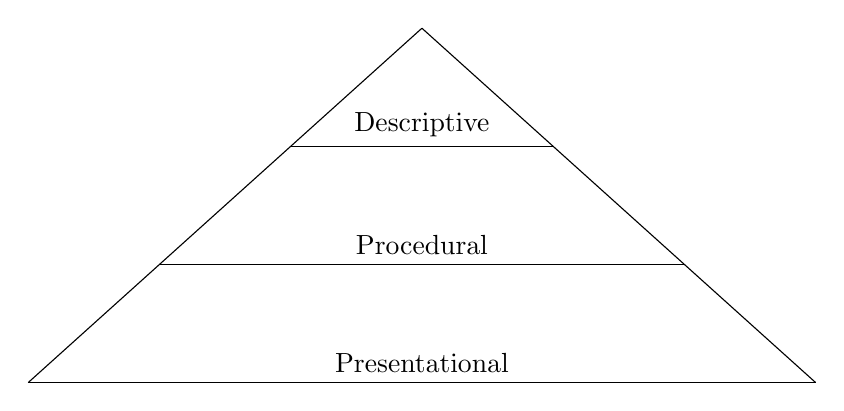
\begin{tikzpicture}
  \coordinate (Descriptive) at (-5,0) {};
  \coordinate (Procedural) at ( 5,0) {};
  \coordinate (Presentational) at ( 0,4.5) {};
  \draw (Descriptive) -- (Presentational);
  \draw (Procedural) -- (Presentational);
  \foreach \y/\Descriptive in {0/Presentational, 1/Procedural, 2/Descriptive} {
      \draw ($(Descriptive)!\y/3!(Presentational)$) -- ($(Procedural)!\y/3!(Presentational)$) node[midway,above] {\Descriptive};
  }
  \end{tikzpicture}

\caption{A hierarchy of markup language abstraction.}
\label{fig:markup-types-hierarchy}
\end{figure}



Consequently I argue that these three ``categories'' of the taxonomy can be viewed as paradigms of markup abstraction. Much like we have invented facilities to abstract away machine level instructions, we have invented facilities to abstract low level instructions for document content transformation. This hierarchy is visualized in Figure \ref{fig:markup-types-hierarchy}.  


% We are talking about _instances_ of documents, which is why we are not regarding abstract markup languages.















\chapter{Workflows}
\label{sec:microframework}
In the spirit of \citet{reid} -- author of the paper that introduced Scribe, one of the earlier document preparation systems that argued for the ``separation of form from content'' -- we will now take a look at some popular workflows of document authoring. Further I will suggest an ideal alternative, targeting some of the apparent deficiencies with the current ones.

The process that we are going to analyze is that of file format transformation. The idea of transforming a file expressed in some format F into some other format F\prim.

Given the creativity of humans, I would argue that, the number of workflows used in the real world today is likely equivalent or higher than the number of people employing a workflow. Thus, in order to be able to discuss workflows, we need some way to generalize the concepts that are present in all. Thus, Figure \ref{fig:workflows-framework} suggests a micro-framework I will use as a basis for this discussion. Given it's high level of abstraction I strongly believe you will agree on it being representative for the whole set of potential workflows.

Think about it, to perform the process described as transforming from \(F\) to \(F\prime\), we obviously need to be able to distinguish the two formats from each other. In Figure \ref{fig:workflows-framework} \(F\) is referred to as ``Input file'' and \(F\prime\) as ``Output file''. Further, we know that \(F\), representing a static file format, never will transform itself into a the other static file format \(F\prime\). Consequently we need some process in-between, in Figure \ref{fig:workflows-framework} we refer to this process as the ``Transformation program''. The figure then, I argue is general enough to encompass every reasonable and imaginable transformation workflow.


\begin{figure}[h]
  \centering

  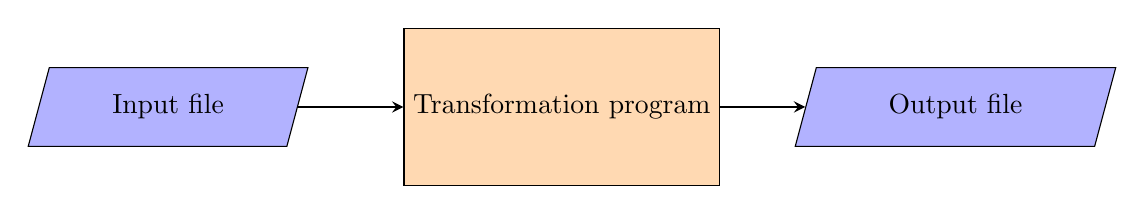
\begin{tikzpicture}[node distance=2.5cm]
    \node (input)  [io] {Input file};
    \node (engine) [process, right of=input, xshift=2.5cm] {Transformation program};
    \node (output) [io,      right of=engine, xshift=2.5cm] {Output file};

    % arrows
    \draw [arrow] (input)  -- (engine);
    \draw [arrow] (engine) -- (output);

    \begin{pgfonlayer}{background}
      % \node [draw, fill=cyan!25, rectangle, rounded corners, fit={(input) (engine) (output)}] { Foobar };
    \end{pgfonlayer}

  \end{tikzpicture}

  \caption{A naive interpretation of the problem of file transformation.}
  \label{fig:workflows-framework}
\end{figure}


You might argue that some workflows actually encompass multiple steps of transformation, and I would of course agree. If you however consider how Figure \ref{fig:workflows-framework} actually depict a function, then it becomes obvious how we could use the output of one function as input to another function. Consequently, it is in the model implicit that you may apply it any number of times.




\paragraph{Generality of a transformation program.}
Unfortunately, the model depicted in Figure \ref{fig:workflows-framework} model is not sufficiently exact for our purposes. With it, we will not be able to illustrate the kind of distinctions we want to depict. Assume that we instead of having the two formats \(F\) and \(F\prime\), have the four formats \(I\), \(I\prime\), \(O\), and \(O\prime\). The two I-based formats are expected to be used as input-formats, and the two O-formats are output formats. Given that the input file in Figure \ref{fig:workflows-framework} represents a single file format, and the same for the output format, then this model cannot possibly encompass this four-format-program.

In order to change the model such that it can depict, what previously in the thesis was referred to as, n-to-n conversions, we will introduce the notion of coupling. In Figure \ref{fig:workflows-framework-spec-in-spec-out} we've introduced a dotted line. This dotted line represents coupling. If any of the components within the area delimited by the dotted line change, the change will ripple through all of the other components. Assume for example that the input file and the transformation program are both within the dotted area. This would mean that to handle a new input we need a new transformation program. Which is of course unwanted.







\section{Common workflows}
We will soon look at some common workflows, and how they can be expressed using the simple micro-framwork described in the previous section. But before we do, let us discuss all the possibilities of coupling in the framework through a quadrant diagram -- depicted in Figure \ref{fig:microframework-quadrant}. Instead of the term coupling we will in the quadrant use the terms ``generalized'' and ``specialized''. To oversimplify -- the first should be considered good and the second bad. The idea is in essence the same as with the previously discussed coupling. If some part of the program is generalized then it would mean that the transformation engine is agnostic to changes in that particular part. If however a particular part is specialized then the transformation program will inevitably have to be rewritten upon changes in the particular part. 


\begin{figure}[h]
  \centering

  \begin{tabular}{r | c | c}
    & \textbf{Generalized output} & \textbf{Specialized output} \\ \hline

    \textbf{Generalized input} &
    A
    &
    B 

    \\ \hline

    \textbf{Specialized input} &
    C
    &
    D
  \end{tabular}

  \caption{All combinations of coupling that can occur in Figure \ref{fig:workflows-framework} expressed in a quadrant diagram}
  \label{fig:microframework-quadrant}
\end{figure}


As you might already have guessed, this thesis is concerned with understanding the eco-system of Quadrant A. Namely the general case. Where input is arbitrary and output is arbitrary. But to really understand what kind of programs fit into this category, and perhaps more importantly -- which ones doesn't -- we will still run through all of the quadrants below, while providing explanations and examples for each.

















\subsection{Specialized in, Specialized out (Quadrant D)}
Programs in Quadrant D (of Figure \ref{fig:microframework-quadrant}) represent the category of really specialized transformers. Programs that convert from one specific input format to some specific output format. The fact that the transformation program is coupled to both the input and the output format essentially means that if want to change input or output format we simply need a new (i.e. another) program.  Programs in this quadrant can be depicted using the micro-framework as in \ref{fig:workflows-framework-spec-in-spec-out}. Such a program could for example be a \LaTeX{} to PDF converter. 

\begin{figure}[p]
  \centering

  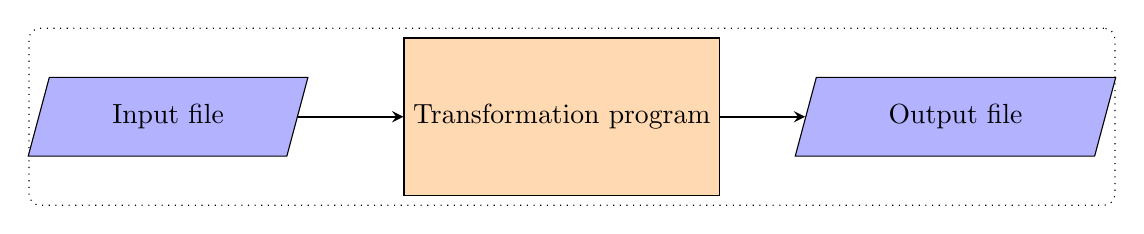
\begin{tikzpicture}[node distance=2.5cm]
    \node (input)  [io] {Input file};
    \node (engine) [process, right of=input, xshift=2.5cm] {Transformation program};
    \node (output) [io,      right of=engine, xshift=2.5cm] {Output file};

    \draw [arrow] (input)  -- (engine);
    \draw [arrow] (engine) -- (output);

    \begin{pgfonlayer}{background}
      \node [dotbox, fit={(input) (engine) (output)}]{};
    \end{pgfonlayer}

  \end{tikzpicture}

  \caption{The dotted line depict coupling, such that if any of the components within the area change, the transformation program must significantly change.}
  \label{fig:workflows-framework-spec-in-spec-out}
\end{figure}



\subsection{Specialized in, Generalized out (Quadrant C)}
Programs in Quadrant C (of Figure \ref{fig:microframework-quadrant}), represent a (to many) very familiar toolset. Namely XML combined with XSLT. The strategy could go something along the following lines. An author express a document in some arbitrary XML format and then use XSLT as a means of outputting multiple different other formats. One could argue that there is a need for one separate XSLT file per output format, or input format. But assuming that the transformation program can be invoked with flags, and that it is written in such a fashion that it supports a wide range of formats, then I would argue it is indeed not coupled. Programs in this quadrant can be depicted using the micro-framework as in \ref{fig:workflows-framework-spec-in-gen-out}.

\begin{figure}[p]
  \centering

  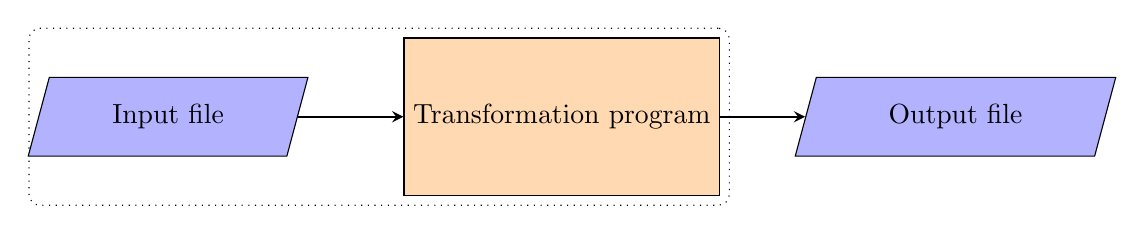
\begin{tikzpicture}[node distance=2.5cm]
    \node (input)  [io] {Input file};
    \node (engine) [process, right of=input, xshift=2.5cm] {Transformation program};
    \node (output) [io,      right of=engine, xshift=2.5cm] {Output file};

    \draw [arrow] (input)  -- (engine);
    \draw [arrow] (engine) -- (output);

    \begin{pgfonlayer}{background}
      \node [dotbox, fit={(input) (engine)}]{};
    \end{pgfonlayer}

  \end{tikzpicture}

  \caption{This Quadrant C program is coupled only to the input format.}
  \label{fig:workflows-framework-spec-in-gen-out}
\end{figure}



\subsection{Generalized in, Specialized out (Quadrant B)}
Programs in Quadrant B (of Figure \ref{fig:microframework-quadrant}) represent a set of very interesting transformation programs. Namely programs that, in theory, take any input, but always convert the output to a fixed kind of output. If an author need a different output format, then he or she simply need to find another program. To be honest I am struggling to find sensible real-world examples for this kind of program. Nevertheless, they are not only interesting, but also highly realizable. Perhaps such a program could be used to convert some set of non-conforming documents to some unified format. For example converting all flavors of miswritten HTML5 into standards-compliant HTML5. Programs in this quadrant can be depicted using the micro-framework as in \ref{fig:workflows-framework-gen-in-spec-out}.

\begin{figure}[p]
  \centering

  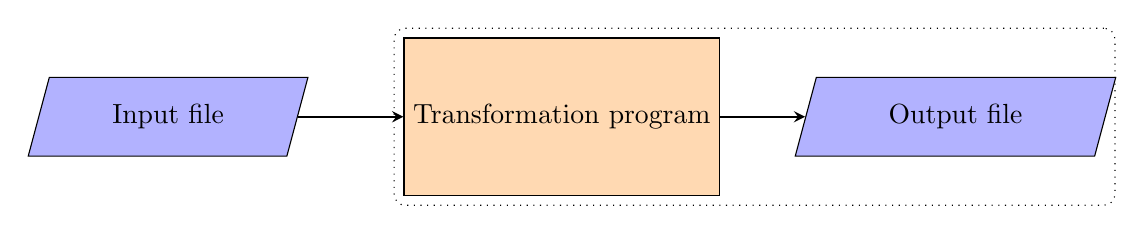
\begin{tikzpicture}[node distance=2.5cm]
    \node (input)  [io] {Input file};
    \node (engine) [process, right of=input, xshift=2.5cm] {Transformation program};
    \node (output) [io,      right of=engine, xshift=2.5cm] {Output file};

    \draw [arrow] (input)  -- (engine);
    \draw [arrow] (engine) -- (output);

    \begin{pgfonlayer}{background}
      \node [dotbox, fit={(engine) (output)}]{};
    \end{pgfonlayer}

  \end{tikzpicture}

  \caption{This Quadrant B program is coupled only to the output format.}
  \label{fig:workflows-framework-gen-in-spec-out}
\end{figure}




\subsection{Generalized in, Generalized out (Quadrant A)}
Programs in Quadrant A (of Figure \ref{fig:microframework-quadrant}) represent the most general kind of programs. They take arbitrary\footnote{As you might have already understood, we are of course not talking about completely arbitrary, but simply multiple unrelated formats.} input formats and generate arbitrary output formats. These are transformation engines that are prepared for taking general input, and providing facilities to give general output. An example program that exhibits this behavior is the widely used software Pandoc.  Programs in this quadrant can be depicted using the micro-framework as in \ref{fig:workflows-framework-gen-in-gen-out}.

\begin{figure}[p]
  \centering

  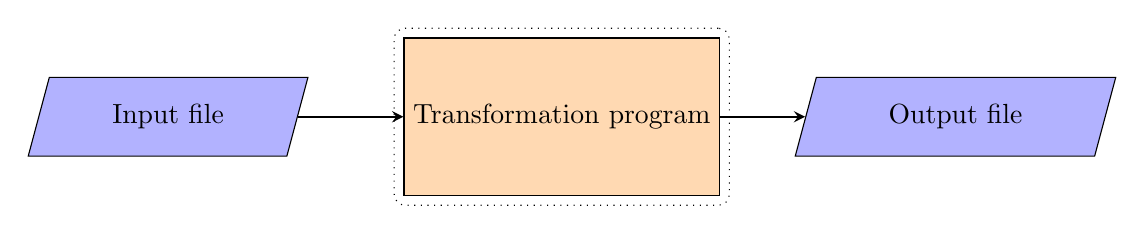
\begin{tikzpicture}[node distance=2.5cm]
    \node (input)  [io] {Input file};
    \node (engine) [process, right of=input, xshift=2.5cm] {Transformation program};
    \node (output) [io,      right of=engine, xshift=2.5cm] {Output file};

    \draw [arrow] (input)  -- (engine);
    \draw [arrow] (engine) -- (output);

    \begin{pgfonlayer}{background}
      \node [dotbox, fit={(engine)}]{};
    \end{pgfonlayer}

  \end{tikzpicture}

  \caption{This Quadrant A program is not coupled to neither input nor output format.}
  \label{fig:workflows-framework-gen-in-gen-out}
\end{figure}







\section{Situational analysis}
In this section we will criticize some of the common workflows through employing the quadrant approach already introduced and depicted by Figure \ref{fig:microframework-quadrant}. \emph{(TODO) I will probably remove this section, because I assume the reader has already appreciated the costs of working outside of the A quadrant.}
% Why are so many documents still procedural?
% Model information flows of contemporary publishing. Figures describing the current state in contrast to the thesis's subjective idea of the ideal state. Refer to Reid (1980).

% \subsection{Presentational}
% i.e. Microsoft Word etc.
% [FIG. ]
% Explicit outline of the problems so that we can attack them in the hypothetical ideal.

% \subsection{Procedural}
% i.e. \LaTeX etc.
% [FIG. ]
% Explicit outline of the problems so that we can attack them in the hypothetical ideal.

% \subsection{Descriptive}
% i.e. DocBook, EPUB, Markdown etc.
% [FIG. ]
% Explicit outline of the problems so that we can attack them in the hypothetical ideal.

% \subsection{A hypothetical ideal addressing the problems}
% [FIG.]

% \subsubsection{Composition \& Abstraction}
% The minimal denominator.











\section{Refining Quadrant A programs}
In order for the model to also encompass the idea of configurability we will extract one piece of the transformation program and thus describe it in further detail. What we will extract is a configuration file (see Figure \ref{fig:workflows-framework-spec-in-spec-out}). Essentially the model of the program can now be seen as a function that takes two arguments and produces one result. An input file, a configuration file that give the end-user some level of control over the transformation process.

We will not introduce any more details now, but instead look at what common workflows we can describe using this model.




\begin{figure}[h]
  \centering

  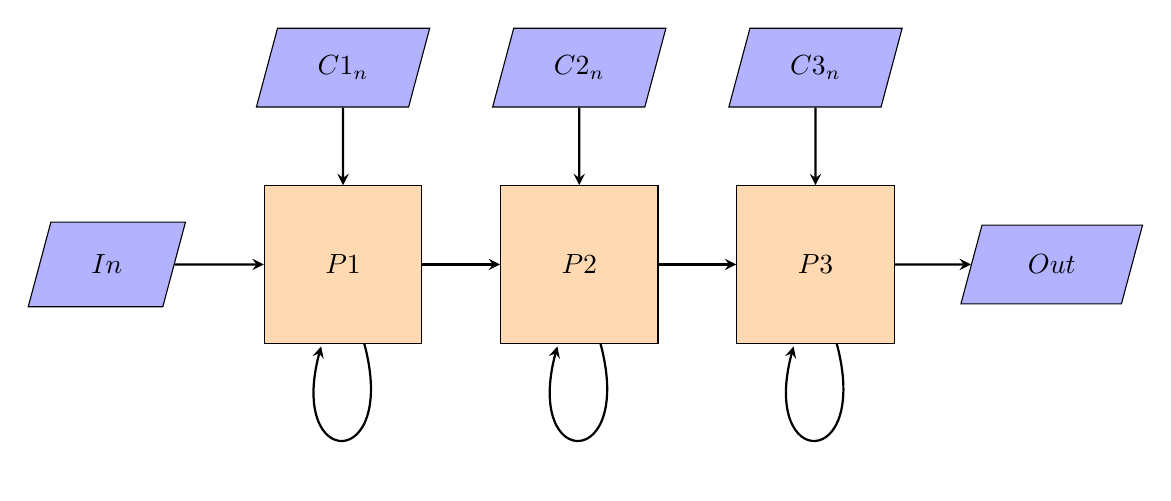
\begin{tikzpicture}[node distance=.5cm]
    \node (in)  [io]                                 {\(In\)};
    \node (P1)  [process, right of=in, xshift=2.5cm] {\(P1\)};
    \node (P2)  [process, right of=P1, xshift=2.5cm] {\(P2\)};
    \node (P3)  [process, right of=P2, xshift=2.5cm] {\(P3\)};
    \node (out) [io,      right of=P3, xshift=2.5cm] {\(Out\)};
    \node (C1)  [io,      above of=P1, yshift=2cm] {\(C1_n\)}; % {Semantics};
    \node (C2)  [io,      above of=P2, yshift=2cm] {\(C2_n\)}; % {Derivations};
    \node (C3)  [io,      above of=P3, yshift=2cm] {\(C3_n\)}; % {Presentation};


    \draw [arrow] (in) -- (P1);
    \draw [arrow] (P1) -- (P2);
    \draw [arrow] (P2) -- (P3);
    \draw [arrow] (P3) -- (out);
    \draw [arrow] (C1) -- (P1);
    \draw [arrow] (C2) -- (P2);
    \draw [arrow] (C3) -- (P3);
    \draw [arrow] (P1) edge[loop below]();
    \draw [arrow] (P2) edge[loop below]();
    \draw [arrow] (P3) edge[loop below]();
  \end{tikzpicture}

  \caption{Suggested ideal refinement of a Quadrant A program.}
  \label{fig:workflows-framework-gen-in-gen-out}
\end{figure}










\chapter{Separating Semantics, Derivations \& Presentation}
TODO.






\chapter{Empirics}
Lorem ipsum.


\section{SimEx -- A control structure-light subset of regex}
...


\section{Flexup -- A DSL for expressing markup-oriented CFG's}
...

\subsection{The annotated file (\texttt{.fup})}
...

\subsection{The annotation definitions file (\texttt{.fupd})}
...

\subsection{The binary}
...





\chapter{Analysis}
Lorem ipsum.





\chapter{Conclusion}
Lorem ipsum.





\chapter{Discussion}
Lorem ipsum.

\section{Future research}
Lorem ipsum.












%
%
% BIBLIOGRAPHY
%
%
\bibliography{bibliography}







\end{document}
